%%
%  ******************************************************************************
%  * #file    Szablon_raportu_EN_Latex.tex
%  * #author  Adrian Wójcik   adrian.wojcik(at)put.poznan.pl
%  *          
%  * #commit  Patryk Kościk   koscikpatryk(at)gmail.com
%  *          Modified the template for Projekt przejsciowy purposes          
%  *          
%  * #version 1.0
%  * #date    09-Mar-2022
%  * #brief   PROJPRZEJ
%  *
%  ******************************************************************************
%%  
\documentclass[11pt, a4paper]{article}

\usepackage{SM_template}

% Wypełnijcie te dyrektywy zgodnie z waszym tematem
% \lab      -> NAZWA CZUJNIKA, np.: 'DHT22'
% \comment  -> Króciutki opis co to, np.: 'Cyfrowy budżetowy czujnik temperatury'
%
\lab{Moduł KY-025}
\comment{Kontaktron, łącznik elektryczny sterowany polem magnetycznym z układem progującym}

% Absolutny zakaz dotykania tego tutaj bo jak dotkiecie to coś jebnie
\university{Politechnika Poznańska}
\faculty{Wydział Automatyki, Robotyki i Elektrotechniki}
\institute{Instytut Robotyki i Inteligencji Maszynowej}
\department{Zakład Sterowania i Elektroniki Przemysłowej}
\addbibresource{bib/Kontaktron-KY-025.bib}
\nocite{*}


%%
%
% Początek dokumentu
%
%%
\begin{document}

%% Strona tytułowa %%
\mainpage{{Kontaktron-KY-025/zdj_modułu/tytulowa.jpg}}
\newpage

\section{Opis elementu} \addcontentsline{toc}{section}{Wstęp}
Zasada działania kontaktronu normalnie zamkniętego, będącego głównym elementem modułu KY-025, polega na oddaleniu od siebie dwóch namagnesowanych styków, znajdujących się wewnątrz szklanej ampułki, przy pomocy zewnętrznego pola magnetycznego (najczęściej jest to po prostu magnes), w konsekwencji rozwierając obwód. 
\vspace{0.3cm}
\begin{figure}[H]
\centering
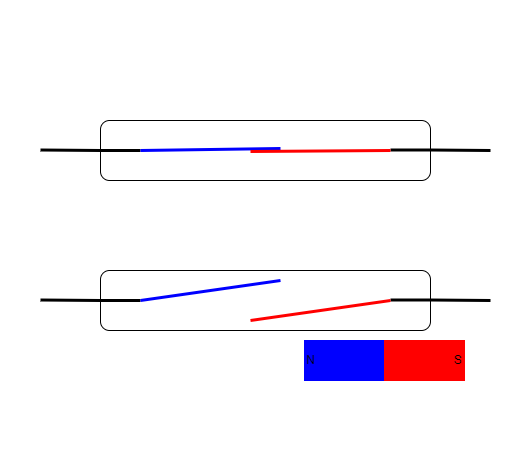
\includegraphics[width=.7\linewidth]{fig/Kontaktron-KY-025/zasada_dzialania/zasada_dzialania.png}
\caption{Działanie kontaktronu normalnie zamkniętego: u góry styki zwarte (brak działania zewnętrznego, silniejszego pola magnetycznego), na dole styki rozwarte (pod wpływem zewnętrznego, silniejszego pola magnetycznego (magnesu))}
\label{fig:sub3}
\end{figure}
\vspace{0.3cm}

\subsection{Opis modułu}
Moduł KY-025 zbudowany jest z kontaktronu normalnie zamkniętego lub normalnie otwartego (opisywany moduł jest z kontaktronem normalnie zamkniętym), potencjometru 100k$\Omega$, układu scalonego LM393 (zawierającego dwa wzmacniacze operacyjne), rezystorów, dwóch diod LED i 4 pinów. Całość jest odpowiednio zamontowana na płytce drukowanej. 
\vspace{0.1cm}
\begin{figure}[H]
\centering
  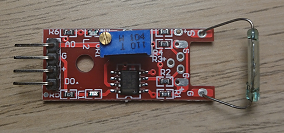
\includegraphics[width=.5\linewidth]{fig/Kontaktron-KY-025/zdj_modułu/widok_z_boku.jpg}
  \caption{Zdjęcie modułu}
  \label{fig:sub1}
\end{figure}
\vspace{0.1cm}
\vspace{0.1cm}
\begin{figure}[H]
\centering
  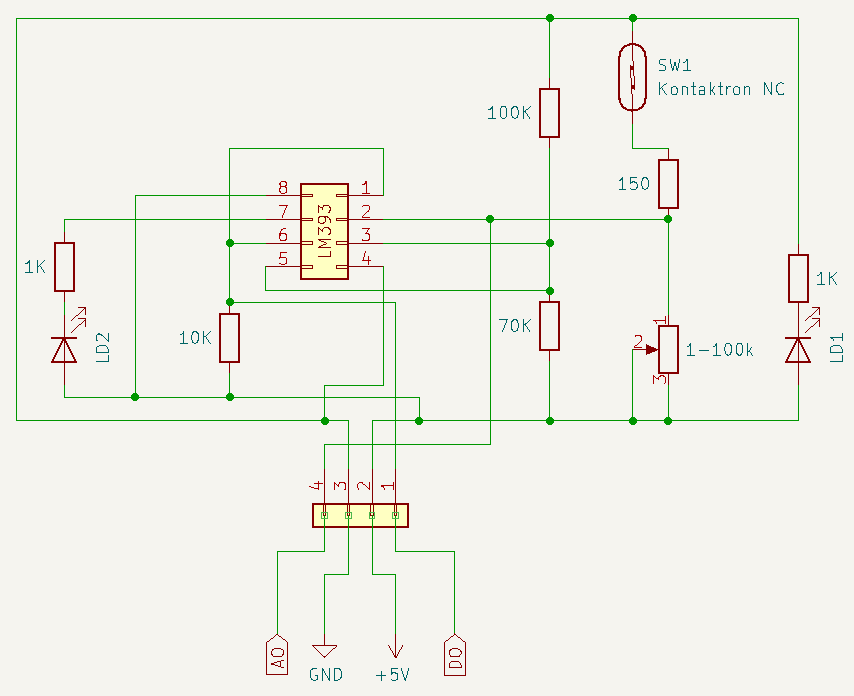
\includegraphics[width=.9\linewidth]{fig/Kontaktron-KY-025/zdj_modułu/schemat_ky_025.png}
  \caption{Schemat modułu}
  \label{fig:sub2}
\end{figure}
\vspace{0.1cm}
% W wyniku rozwarcia styków na wyjściu cyfrowym pojawia się sygnał odpowiadający logicznemu stanowi "1" (w przypadku KY-025 jest to ok. 97\% wartości napięcie zasilania), natomiast na wyjściu analogowym pojawi się napięcie o wartości zależnej od rezystancji ustawionej na potencjometrze.

\subsection{Zastosowania}
Najczęstszym zastosowaniem modułów kontaktronowych są systemy alarmowe, w których kontaktron umieszcza się na oknach/drzwiach. W momencie ich otwarcia obwód zmienia swój stan (jest rozwierany/zamykany), co jest rejestrowane przez odpowiedni system. Innym zastosowaniem jest szeroko pojęta robotyka i automatyka przemysłowa, gdzie kontaktronów używa się do pozycjonowania ramienia robotycznego lub taśmociągu.


\newpage
\hypersetup{
    colorlinks=true,
    linkcolor=blue,
    filecolor=magenta,      
    urlcolor=cyan,
    pdftitle={Overleaf Example},
    pdfpagemode=FullScreen,
    }
\section{Użycie czujnika}
Na podstawie schematu z Rys.\ref{fig:sub2} można wywnioskować, że LED LD1 informuje o załączeniu zasilania w module. W przypadku elementu z kontaktronem normalnie zamkniętym, zaraz po połączeniu zasilania zapali się również dioda LED LD2 odpowiedzialna za pokazywanie stanu przewodzenia prądu przez kontaktron (zapalona dioda - kontaktron zamyka obwód - płynie prąd). 
\vspace{0.2cm}
\begin{figure}[H]
\centering
\includegraphics[width=.9\linewidth]{fig/Kontaktron-KY-025/działanie_ukladu/vcc_nc.JPG}
\caption{Stan układu po połączeniu jedynie zasilania, widać zapalone obie diody LED, zgodnie z opisem}
\label{fig:sub3}
\end{figure}
\vspace{0.2cm}
\vspace{0.2cm}
\begin{figure}[H]
\centering
\begin{subfigure}{.5\textwidth}
  \centering
  \includegraphics[width=.9\linewidth]{fig/Kontaktron-KY-025/zasada_dzialania/DSC_0151.JPG}
  \label{fig:sub1}
  \caption{Mierzone napięcie wyjścia cyfrowego tylko przy połączeniu zasilania}
\end{subfigure}%
\begin{subfigure}{.5\textwidth}
  \centering
  \includegraphics[width=.9\linewidth]{fig/Kontaktron-KY-025/zasada_dzialania/DSC_0152.JPG}
  \label{fig:sub1}
  \caption{Mierzone napięcie wyjścia analogowego tylko przy połączeniu zasilania}
\end{subfigure}
%\caption{}
\label{fig:test}
\end{figure}
\vspace{0.2cm}
Powyższa sytuacja ma wyjaśnienie w schemacie z Rys.\ref{fig:sub2}. Wyjście cyfrowe jest podłączone do wyjścia komparatora (zawartego w układzie scalonym LM393, styk nr 1), a wyjście analogowe do rozdzielnika napięcia , który łączy się z wejściem ujemnym komparatora. W momencie gdy zamknięty jest kontaktron, znaczna część napięcia zasilania (ponad 99.8\%) zostanie rozproszona na potencjometrze, co spowoduje, że napięcie znajdujące się na wyjściu A0 będzie pomijalnie małe. W konsekwencji na wyjściu komparatora znajdzie się wzmocniona (w teorii do nieskończoności, w praktyce ogarniczona napięciem zasilania wzmacniacza operacyjnego) różnica napięć wejściowych, która da na wyjściu cyfrowym stan logiczny "1".

% \vspace{0.5cm}
% \begin{figure}[H]
% \centering
% \begin{subfigure}{.5\textwidth}
%   \centering
%   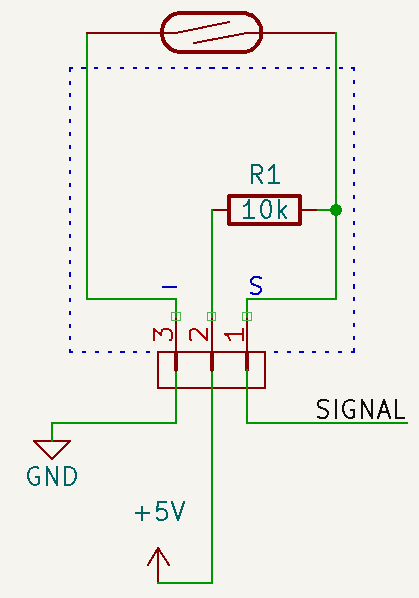
\includegraphics[width=.5\linewidth]{fig/Kontaktron-KY-025/polaczenie_modulu/podciagajacy.png}
%   \label{fig:sub1}
%   \caption{Wariant połączenia pull-up}
% \end{subfigure}%
% \begin{subfigure}{.5\textwidth}
%   \centering
%   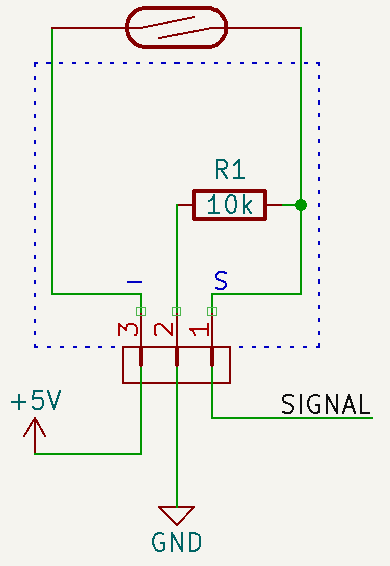
\includegraphics[width=.5\linewidth]{fig/Kontaktron-KY-025/polaczenie_modulu/sciagajacy.png}
%   \label{fig:sub2}
%   \caption{Wariant połączenia pull-down}
% \end{subfigure}
% \caption{Połączenie elektryczne}
% \label{fig:test}
% \end{figure}
% \vspace{0.5cm}


\section{Prezentacja działania układu}
W celu zaprezentowania działania układu wgrano na mikrokontroler program, który przyjmuje na swoje wejście GPIO wartość wyjścia cyfrowego czujnika i po wykryciu obecności stanu wysokiego zapala niebieską diodę użytkownika. Zostało to zaprezentowane w tym filmie \cite{youtube} i na zdjęciach poniżej. 

\vspace{0.2cm}
\begin{figure}[H]
\centering
\begin{subfigure}{.5\textwidth}
  \centering
  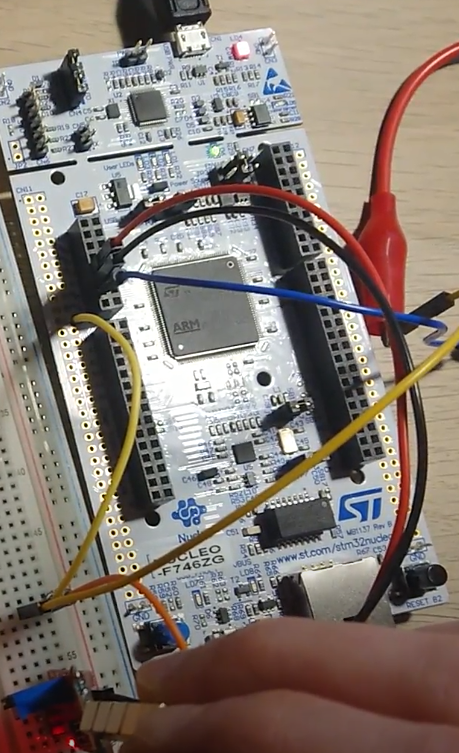
\includegraphics[width=.9\linewidth]{fig/Kontaktron-KY-025/działanie_ukladu/zwarty.PNG}
  \label{fig:sub1}
  %\caption{Mierzone napięcie wyjścia cyfrowego tylko przy połączeniu zasilania}
\end{subfigure}%
\begin{subfigure}{.5\textwidth}
  \centering
  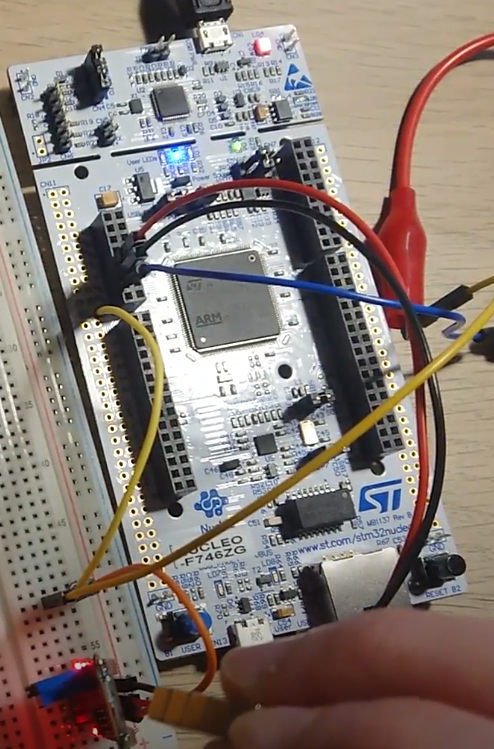
\includegraphics[width=0.97\linewidth]{fig/Kontaktron-KY-025/działanie_ukladu/rozwarty.PNG}
  \label{fig:sub1}
  %\caption{Mierzone napięcie wyjścia analogowego tylko przy połączeniu zasilania}
\end{subfigure}
\caption{Zdjęcie po lewo - kontaktron rozwarty, na wejście GPIO nie jest kierowany sygnał, dioda użytkownia LD2 się nie świeci. Zdjęcie po prawo - kontaktron zwarty, na wejście GPIO jest kierowany sygnał, dioda użytkownia LD2 się świeci}
\label{fig:test}
\end{figure}
\vspace{0.2cm}

\newpage
W module znajduje się także układ progujący, zrealizowany przy pomocy komparatora i potencjometru, który reguluje wartośc napięcia na wyjściu analogowym układu. Ze względu na charakterystykę potencjometru (zakres do 100k$\Omega$, zmiana rezystancji ok. 100$\Omega$/obrót) prezentacja tej zmiany na nagraniu jest problematyczna, więc została ona pokazana na zdjęciach poniżej.

\vspace{0.2cm}
\begin{figure}[H]
\centering
\includegraphics[width=.7\linewidth]{fig/Kontaktron-KY-025/działanie_ukladu/DSC_0157.JPG}
\caption{Napięcie na wyjściu analogowym 4.92V}
\label{fig:sub3}
\end{figure}
\vspace{0.2cm}
\vspace{0.2cm}
\begin{figure}[H]
\centering
\includegraphics[width=.7\linewidth]{fig/Kontaktron-KY-025/działanie_ukladu/DSC_0161.JPG}
\caption{Napięcie na wyjściu analogowym po zmianie rezystancji potencjometru - 4.96V}
\label{fig:sub3}
\end{figure}
\vspace{0.2cm}

\printbibliography[heading=bibintoc]

\end{document}